\begin{figure}[H]
    \centering



\tikzset{every picture/.style={line width=0.75pt}} %set default line width to 0.75pt        

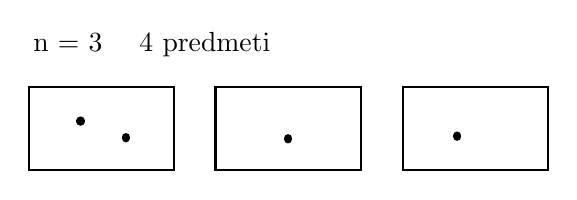
\begin{tikzpicture}[x=0.75pt,y=0.75pt,yscale=-1,xscale=1]
%uncomment if require: \path (0,300); %set diagram left start at 0, and has height of 300

%Shape: Rectangle [id:dp7407184316163662] 
\draw   (90.25,90.25) -- (160.25,90.25) -- (160.25,130.25) -- (90.25,130.25) -- cycle ;
%Shape: Rectangle [id:dp5723531652661165] 
\draw   (180.25,90.25) -- (250.25,90.25) -- (250.25,130.25) -- (180.25,130.25) -- cycle ;
%Shape: Rectangle [id:dp06732545223532949] 
\draw   (270.5,90.25) -- (340.5,90.25) -- (340.5,130.25) -- (270.5,130.25) -- cycle ;
%Shape: Free Drawing [id:dp5149127238979943] 
\draw  [line width=3] [line join = round][line cap = round] (115.25,106.76) .. controls (115.25,106.59) and (115.25,106.43) .. (115.25,106.26) ;
%Shape: Free Drawing [id:dp5804075845098335] 
\draw  [line width=3] [line join = round][line cap = round] (137,114.76) .. controls (137,114.59) and (137,114.43) .. (137,114.26) ;
%Shape: Free Drawing [id:dp5627736685120888] 
\draw  [line width=3] [line join = round][line cap = round] (215.25,115.26) .. controls (215.25,115.09) and (215.25,114.93) .. (215.25,114.76) ;
%Shape: Free Drawing [id:dp5538210827206191] 
\draw  [line width=3] [line join = round][line cap = round] (296.75,114.01) .. controls (296.75,113.84) and (296.75,113.68) .. (296.75,113.51) ;

% Text Node
\draw (91,62) node [anchor=north west][inner sep=0.75pt]   [align=left] {n = 3 \ \ \ 4 predmeti};


\end{tikzpicture}
    
\end{figure}